\documentclass{article}
\usepackage[utf8]{inputenc}
\usepackage{amsmath}
\usepackage{amssymb}
\usepackage{mathtools}
\usepackage{graphicx}
\graphicspath{{Images/}}

\setlength{\oddsidemargin}{0in}
\setlength{\textwidth}{6.5in}
\setlength{\topmargin}{-.55in}
\setlength{\textheight}{9in}
\pagestyle{empty}


\title{Scientific Computation II HW1}
\author{Michael Nameika}
\date{January 2023}

\begin{document}

\maketitle

\section*{Problem 1.4}

Run Program 1 to $N = 2^{16}$ instead of $2^{12}$. What happens to the plot of error vs. $N$? Why? Use the Matlab commands tic and toc to generate a plot of approximately how the computation time depends on $N$. Is the dependence linear, quadratic, or cubic?
\newline\newline
Running Program 1 to $N=2^{16}$, we see that the error begins to increase for larger values of $N$. This occurs because of machine round-off error.
\newline
\begin{center}
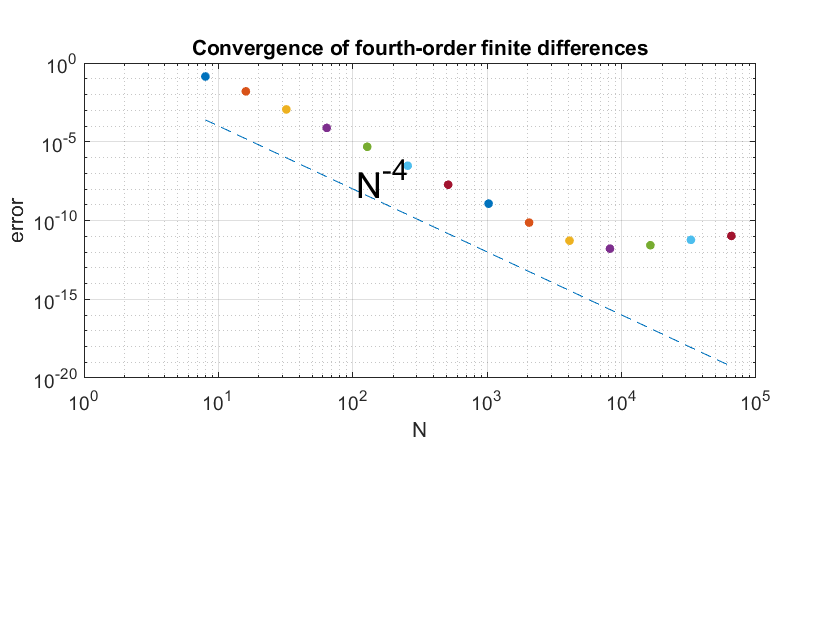
\includegraphics[scale = 0.5]{problem 1 plot 1 sci comp.png}
\end{center}

Notice in the plot below the dependence appears to be more quadratic than anything. 
\newline
\begin{center}
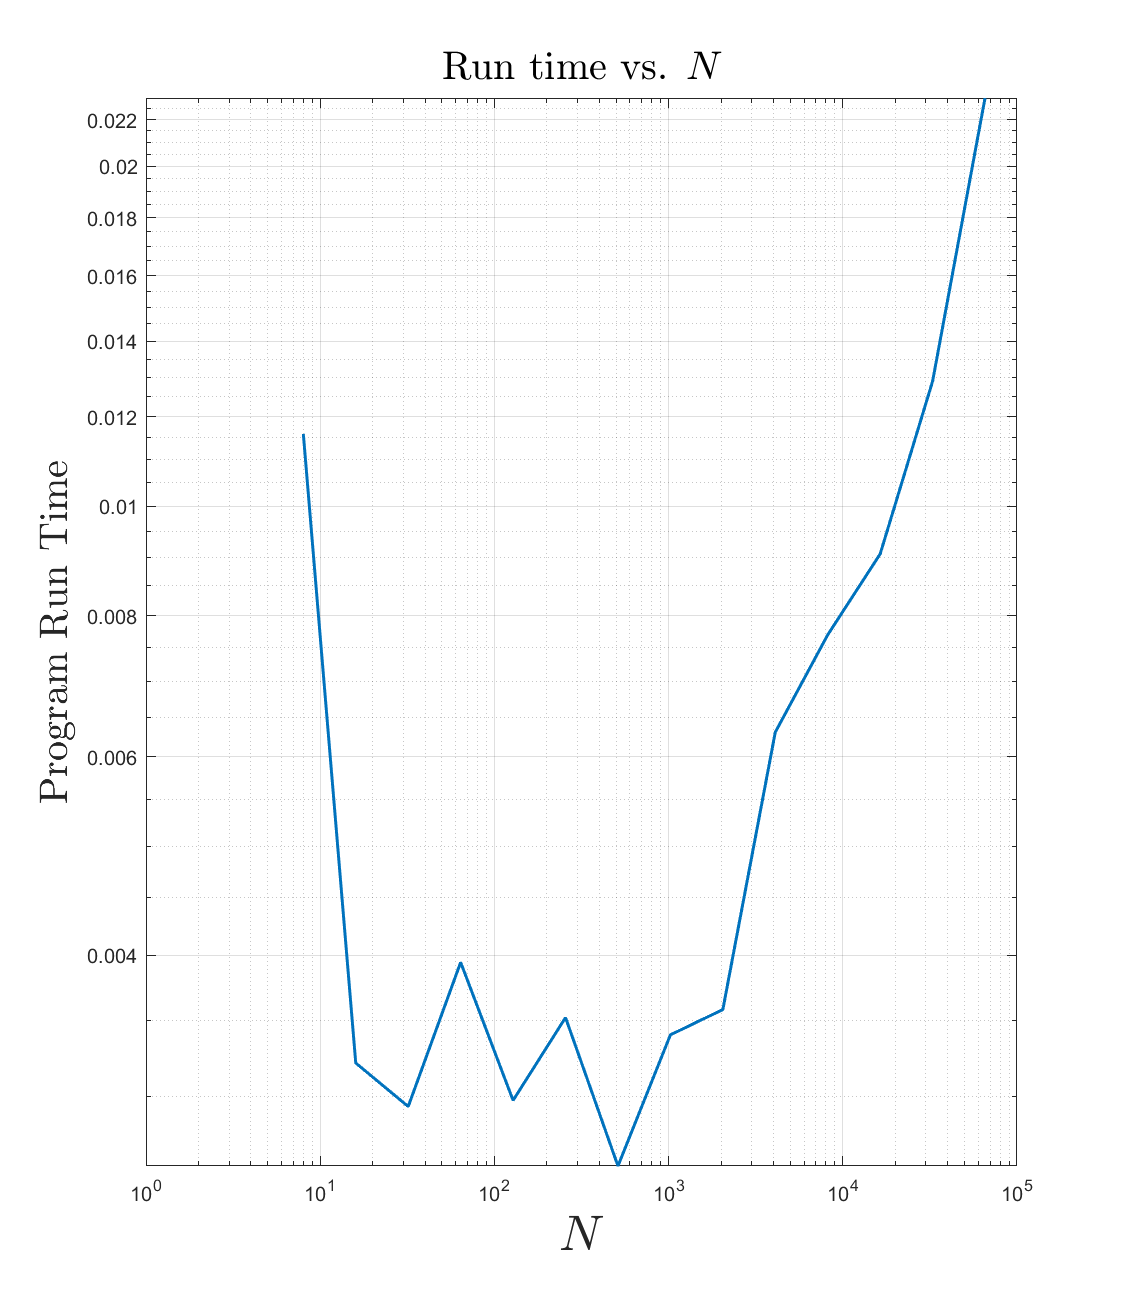
\includegraphics[scale = 0.4]{Problem 1 plot sci comp.png}
\end{center}

Note: run time is in seconds.


\section*{Problem 1.5}

Run Programs 1 and 2 with $e^{\sin(x)}$ replaced by (a) $e^{\sin^2(x)}$ and (b) $e^{\sin(x)|\sin(x)|}$ and with uprime adjusted appropriately. What rates of convergence do you observe? Comment.
\newline\newline
\begin{itemize}
    \item[(a)] Notice for $u(x) = e^{\sin^2(x)}$, $u'(x) = \sin(2x)u(x)$. Replacing $u$ and uprime in program 1 and 2 with this, we find the following rate of convergence: 
    \newline
    \begin{center}
        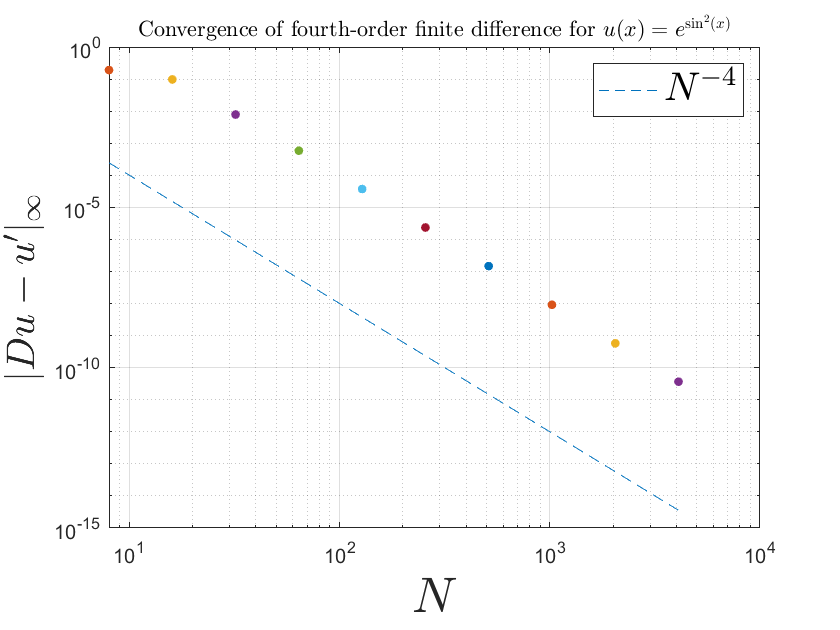
\includegraphics[scale =0.4]{expsin2.png}
    \end{center}
    And for the spectral differentiation matrix, we find the following plot of convergence:
    \begin{center}
        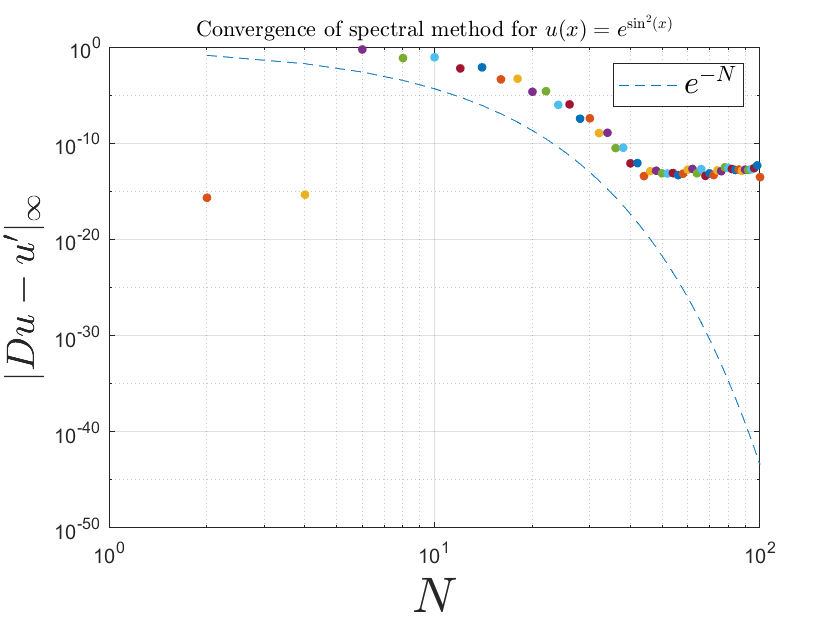
\includegraphics[scale = 0.4]{spectral expsin2 with exp.png}
    \end{center}

    Notice for the first program, the rate of convergence is approximately $\mathcal{O}(h^4)$ whereas the spectral method has exponential convergence until it very rapidly reaches machine precision.
    
    \item[(b)] Notice for $u(x) = e^{\sin(x)|\sin(x)|}$, $u'(x) = 2\cos(x)|\sin(x)|e^{\sin(x)|\sin(x)|}$. Replacing $u$ and uprime in programs 1 and 2 with the above, we find the following plots of convergence:
    \newline
    \begin{center}
        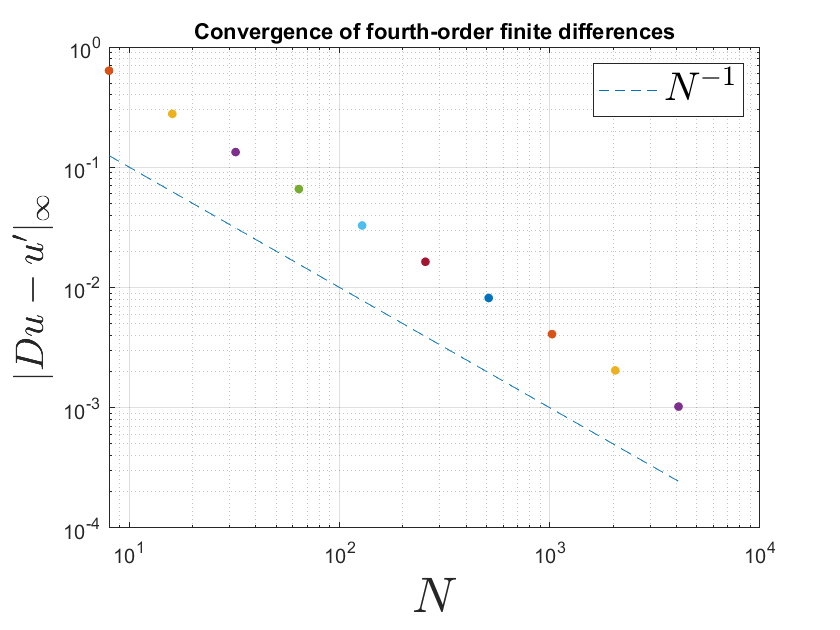
\includegraphics[scale = 0.4]{expsinabssin.png}
    \end{center}
    And for the spectral differentiation method, we find
    \begin{center}
        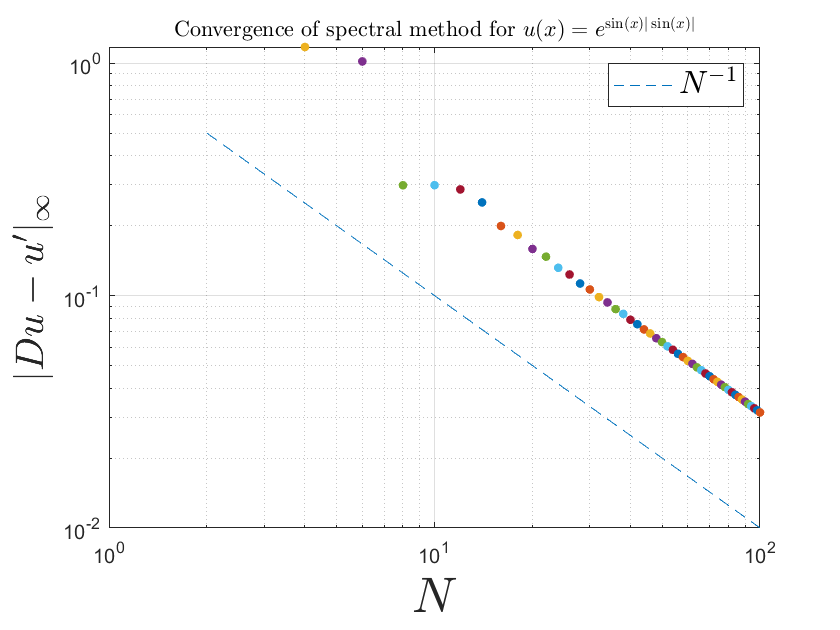
\includegraphics[scale = 0.4]{spectral expsinabssin.png}
    \end{center}
    Notice in this case that both methods are approximately first order accurate. The difference in order of accuracy between these two methods is due to the fact that $u$ has only one continuous derivative.
    \begin{center}
        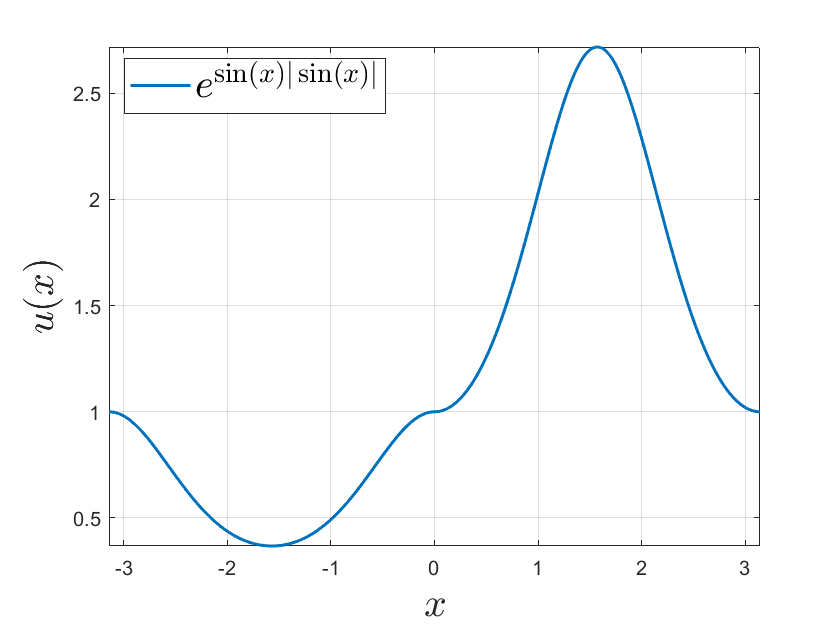
\includegraphics[scale = 0.3]{plot exp_sin_abs_sin.png}
        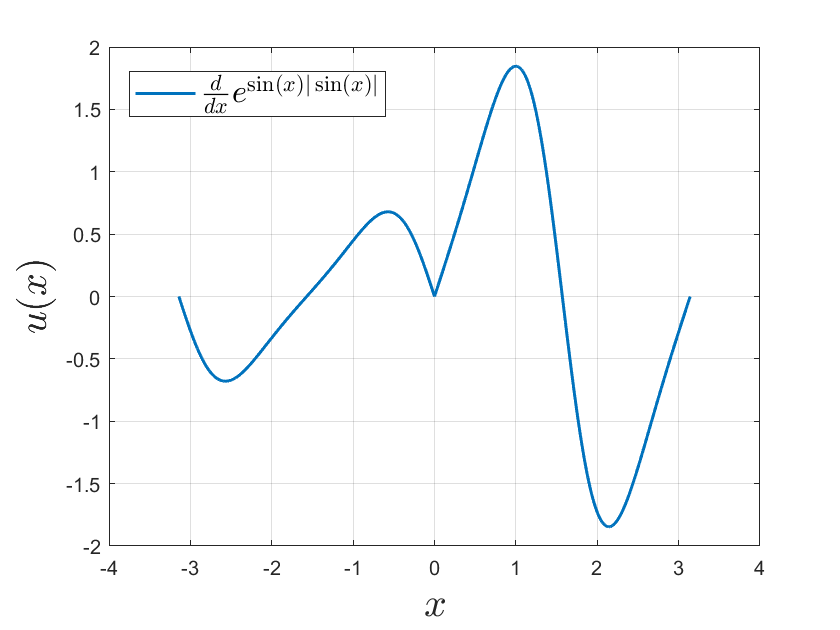
\includegraphics[scale = 0.3]{uprimemm.png}
    \end{center}

\end{itemize}


\section*{Problem 1.6}
By manipulating Taylor series, determine the constant $C$ for an error expansion of (1.3) of the form $w_j - u'(x_j) \sim Ch^4u^{(5)}(x_j)$, where $u^{(5)}$ denotes the fifth derivative. Based on this value of $C$ and on the formula for $u^{(5)}(x)$ with $u(x) = e^{\sin(x)}$, determine the leading term in the expansion for $w_j - u'(x_j)$ for $u(x) = e^{\sin(x)}$. (You will have to find $\max_{x \in [-\pi, \pi]}|u^{(5)}(x)|$ numerically.) Modify Program 1 so that it plots the dashed line corresponding to this leading term rather than just $N^{-4}$. This adjusted dashed line should fit the data almost perfectly. Plot the difference between the two on a log-log scale and verify that it shrinks at the rate $\mathcal{O}(h^6)$.
\newline\newline
From (1.3), we have the following fourth order method in matrix notation:
\[
\begin{pmatrix}
    w_1 \\
    \\
    \\
    \\
    \\
    \vdots\\
    \\
    \\
    \\
    w_N\\

\end{pmatrix}
= h^{-1}\begin{pmatrix}
    & & \ddots & & & \frac{1}{12} & -\frac{2}{3} \\
    & & \ddots & -\frac{1}{12} & & & \frac{1}{12} \\
    & & \ddots & \frac{2}{3} & \ddots \\
    & & \ddots & 0 & \ddots \\
    & & \ddots & -\frac{2}{3} & \ddots \\
    -\frac{1}{12} & & & \frac{1}{12} & \ddots \\
    \frac{2}{3} & -\frac{1}{12} & & & \ddots \\
\end{pmatrix}
\begin{pmatrix}
    u_1\\
    \\
    \\
    \\
    \\
    \vdots\\
    \\
    \\
    \\
    u_N\\
\end{pmatrix}
\]
From this, we can see, for $w_j$:
\[w_j = \frac{1}{h}\left(\frac{1}{12}u_{j-2} - \frac{2}{3}u_{j-1} + \frac{2}{3}u_{j+1} - \frac{1}{12}u_{j+2}\right)\]
Taylor expanding $u_{j-2}$, $u_{j-1}$, $u_{j+1}$, and $u_{j+2}$, we find
\begin{align*}
    u_{j-2} &= u_j - 2hu_j' + 2h^2u_j'' - \frac{8h^3}{3!}u_j''' + \frac{16h^4}{4!}u_j^{(4)} - \frac{32h^5}{5!}u_j^{(5)} + \mathcal{O}(h^6) \\
    u_{j-1} &= u_j - hu_j' + \frac{h^2}{2}u_j'' - \frac{h^3}{3!}u_j''' + \frac{h^4}{4!}u_j^{(4)} - \frac{h^5}{5!}u_j^{(5)} + \mathcal{O}(h^6) \\
    u_{j+1} &= u_j + hu_j' + \frac{h^2}{2}u_j'' + \frac{h^3}{3!}u_j''' + \frac{h^4}{4!}u_j^{(4)} + \frac{h^5}{5!}u_j^{(5)} + \mathcal{O}(h^6) \\
    u_{j+2} &= u_j + 2hu_j' + 2h^2u_j'' + \frac{8h^3}{3!}u_j''' + \frac{16h^4}{4!}u_j^{(4)} + \frac{32h^5}{5!}u_j^{(5)} + \mathcal{O}(h^6) \\
\end{align*}
then
\begin{align*}
    u_{j+1} - u_{j-1} &= 2hu_j' + \frac{2h^3}{3!}u_j''' + \frac{2h^5}{5!}u_j^{(5)} + \mathcal{O}(h^6)\\
    u_{j-2} - u_{j+2} &= -4hu_j' - \frac{16h^3}{3!}u_j''' - \frac{64h^5}{5!}u_j^{(5)} + \mathcal{O}(h^6)\\
    \\
    \frac{2}{3}\left(u_{j+1} - u_{j-1}\right) &= \frac{4h}{3}u_j' + \frac{2h^3}{9}u_j''' + \frac{h^5}{90}u_j^{(5)} + \mathcal{O}(h^6) \\
    \frac{1}{12}\left(u_{j-2} - u_{j+2}\right) &= -\frac{h}{3}u_j' - \frac{2h^3}{9}u_j''' - \frac{32h^5}{5}u_j^{(5)}\ + \mathcal{O}(h^6)\\
\end{align*}
and finally, 
\begin{align*}
    w_j - u_j' &= \frac{1}{h}\left(\frac{1}{12}(u_{j-2}-u_{j+2}) + \frac{2}{3}(u_{j+1} - u_{j-1})\right) - u_j' \\
    &= -\frac{h^4}{30}u_j^{(5)} \\
\end{align*}
Thus, the constant $C$ is $C = \frac{1}{30}$. Additionally, numerically differentiating $e^{\sin(x)}$ five times, we find the maximum on $x\in [-\pi, \pi]$ to be $\max_{x\in [-\pi, \pi]} \frac{d^5}{dx^5}e^{\sin(x)} \approx 24.31$. Modifying Program 1 to include this, we find the following plot for the error of convergence:
\begin{center}
    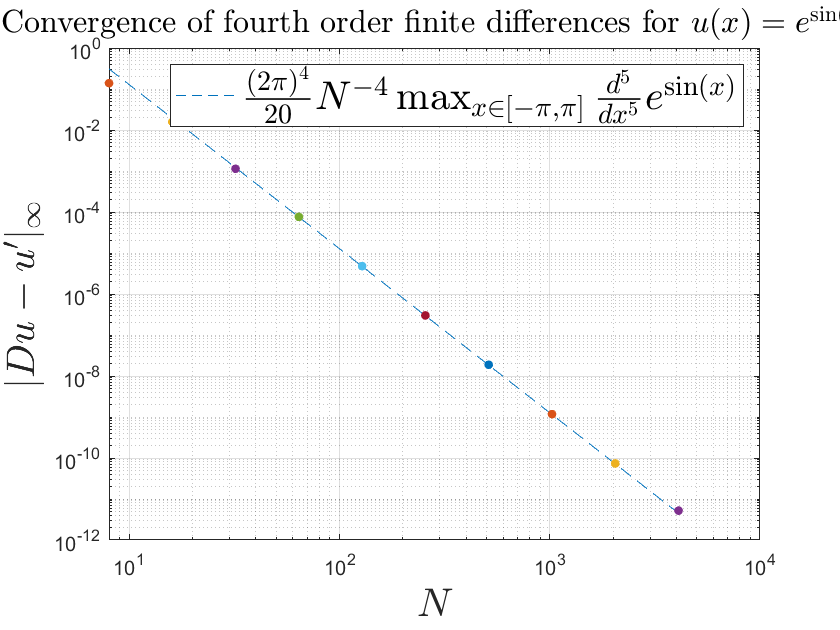
\includegraphics[scale = 0.6]{correctedError.png}
\end{center}
Notice how well the adjusted line fits the data!

\section*{Problem 2.6}
We obtained the entries of (1.4) by differentiating the sinc function. Derive the same result by calculating the inverse semidiscrete Fourier transform of $ik\hat{\delta}(k)$.
\newline\newline
Recall that $\hat{\delta}(k) = h$ for all $k \in [-\pi/h, \pi/h]$ and that the inverse semidiscrete Fourier transform is given by the following equation:
\[v_j = \frac{1}{2\pi}\int_{-\pi/h}^{\pi/h}e^{ikx_j}\hat{v}(k)dk, \;\;\;\; j \in \mathbb{Z}\]
Then we have the inverse semidiscrete Fourier transform of $ik\hat{\delta}(k)$ is
\begin{align*}
    \frac{1}{2\pi}\int_{-\pi/h}^{\pi/h}e^{ikx_j}ik\hat{\delta}(k)dk &= \frac{1}{2\pi}\int_{-\pi/h}^{\pi/h}e^{ikx_j}ikhdk \\
    &= \frac{ih}{2\pi}\int_{-\pi/h}^{\pi/h}ke^{ikx_j}dk \\
    &= \frac{ih}{2\pi}\left[\frac{\pi}{ihx_j}(e^{ix_j\pi/h} + \frac{\pi}{ihx_j}e^{-ix_j\pi/h}) + \frac{1}{x_j^2}(e^{ix_j\pi/h} - e^{-ix_j\pi/h})\right] \\
    &= \frac{ih}{2\pi}\left[\frac{\pi}{ih^2j}(2\cos(\pi j)) + \frac{2j}{j^2h^2}\sin(\pi j)\right] \\
    &= \frac{(-1)^j}{hj} \\
\end{align*}
Which is what we sought to show.

\section*{Problem 2.7}
Modify Program 3 to determine the maximum error over $\mathbb{R}$ in the sinc function interpolants of the square wave and the hat function, and to produce a log-log plot of these two error maxima as functions of $h$. (Good choices for $h$ are $2^{-3}$, $2^{-4}$, $2^{-5}$, $2^{-6}$.) What convergence rates do you observe as $h \to 0$?
\newline\newline
For the delta function and square wave, as we can see below, the convergence is virtually nonexistent. That is, as the value of $h$ decreases, the error did not appear to improve. However, for the hat function, we appear to get first order convergence as $h \to 0$.
\begin{center}
    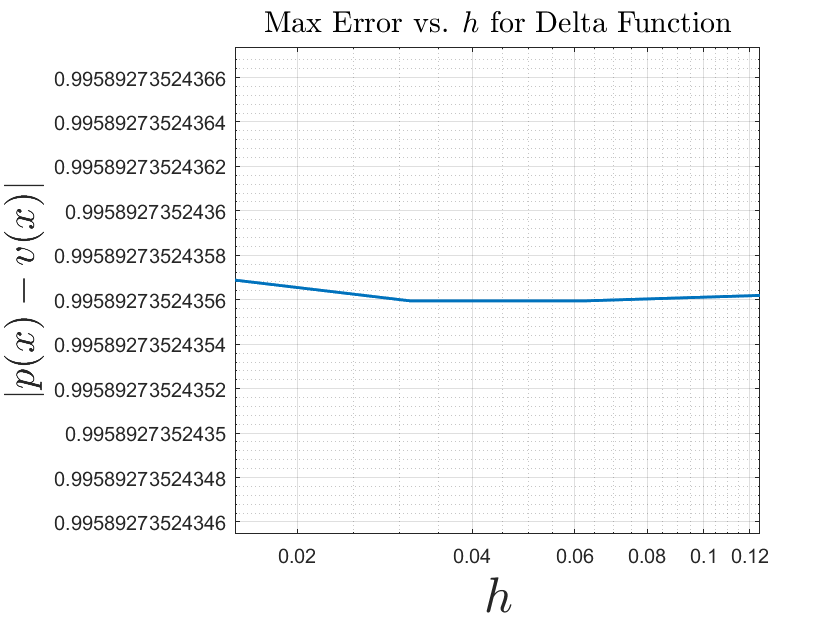
\includegraphics[scale = 0.3]{deltafunctionHerr.png}
    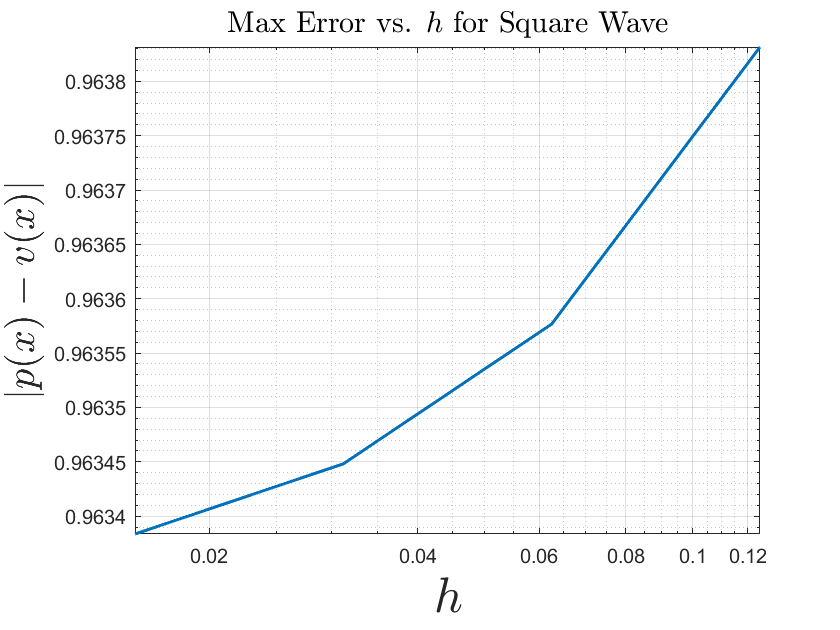
\includegraphics[scale = 0.3]{squarewaveHerr.png}
    \newline
    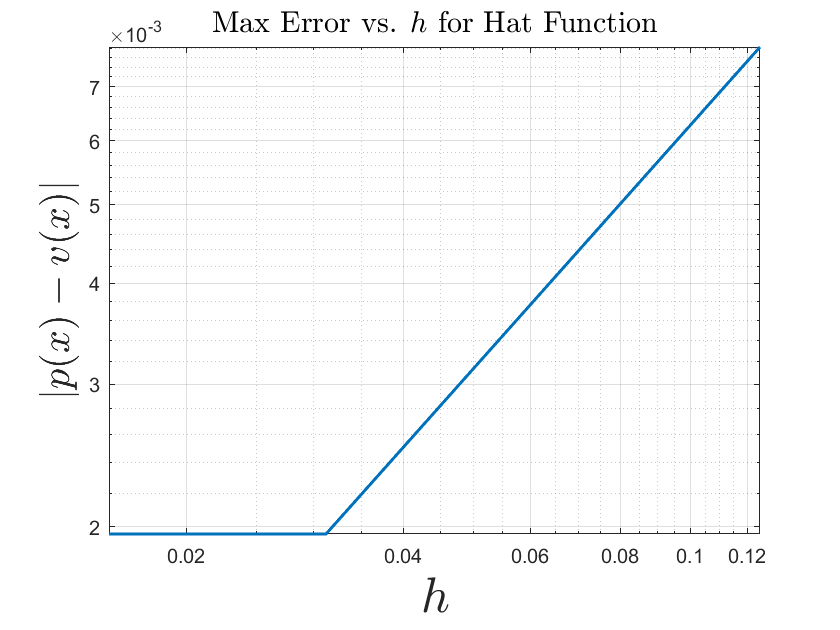
\includegraphics[scale = 0.4]{hatfunctionHplot.png}
\end{center}

\section*{Problem 3.5}
Using the commands tic and toc, study the time taken by MATLAB (which is far from optimal in this regard) to compute an $N$-point FFT, as a function of $N$. If $N=2^k$ for $k=0,1,\dots,15$, for example, what is the dependence of the time on $N$? What if $N=500,501, \dots, 519, 520$? From a plot of the latter results, can you spot the prime numbers in this range? (\textit{Hints}. The commands isprime and factor may be useful. To get good tic/toc data it may help to compute each FFT 10 or 100 times in a loop.)
\newline\newline
Running the MATLAB built in FFT command on the function
\[f(x) = 0.7\sin(100\pi x) + \sin(240\pi x)\]
on the interval $x \in [0, 2\pi]$ with $N = 2^k$ for $k=0,1,\dots, 15$, 100 times for each $k$ value, we find the following plot of the time for the command to run versus $N$:
\begin{center}
    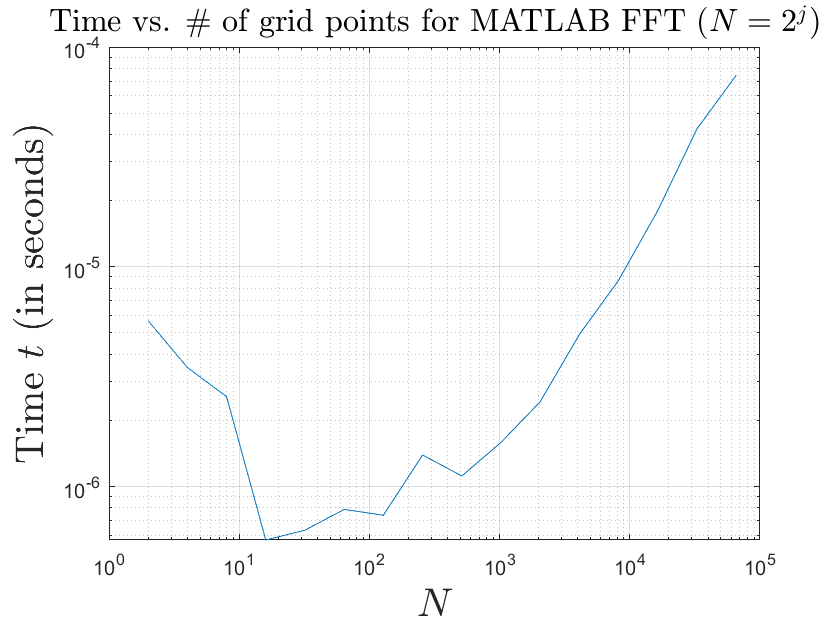
\includegraphics[scale = 0.44]{powersof2fft.png}
\end{center}
Running the built in MATLAB FFT command for the same function on the same interval with $ = 500,501,\dots 519,520$ 100 times, we find the following plot of the time for the command to run versus $N$:
\begin{center}
    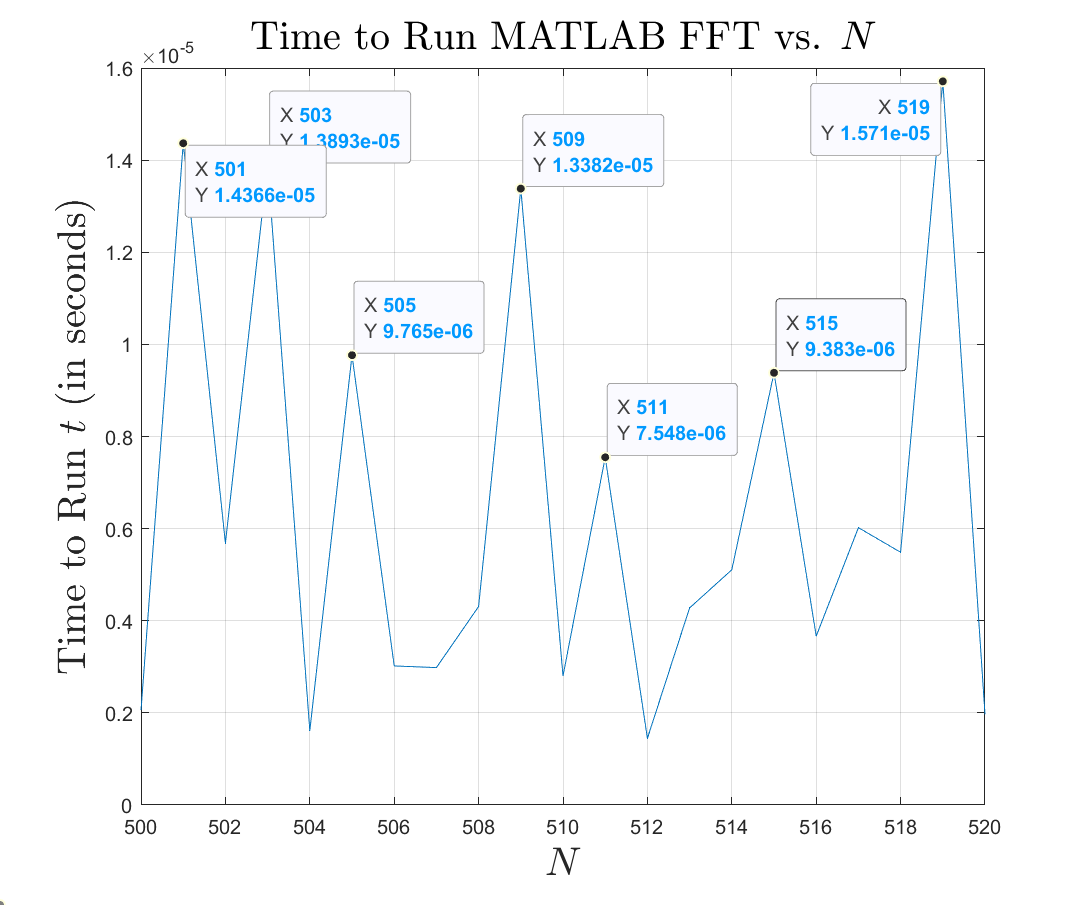
\includegraphics[scale = 0.45]{Images/timetoRunFFT.png}
\end{center}
Notice that spikes in the computation time occur at $N$ values of 501, 503, 505, 509, 511, 515, and 519. From this list, 503, 509 are prime. Additionally, the other numbers in the list factor into the product of two primes, as we can see in the table below:
\newline
\begin{center}
    \begin{tabular}{c|c}
        Number & Prime Factorization \\
        \hline
        501 & $3\times 167$ \\
        505 & $5 \times 101$ \\
        511 & $7\times 73$ \\
        515 & $5\times 103$ \\
        519 & $3\times 173$ \\
    \end{tabular}
\end{center}

\section*{Problem 3.6}
We have seen that a discrete function $v$ can be spectrally differentiated by means of two complex FFTs (one forward, one inverse). Explain how two distinct discrete functions $v$ and $w$ can be spectrally differentiated at once by the same two complex FFTs, provided that $v$ and $w$ are real.
\newline\newline
Suppose $v$ and $w$ are both real, discrete functions. We may spectrally differentiate both $v$ and $w$ at once by defining 
\[y  = v + iw\]
and finding the Fourier transform of $y$, differentiating, and evaluating the inverse Fourier transform and separating the real and imaginary components of the result to recover the spectral derivative of $v$ and $w$. See the following flowchart:
\[(y = v + iw) \:\: \xrightarrow{\text{FFT}} \:\: \hat{y} \:\: \xrightarrow{\text{S.D.}} \:\: ik\hat{y} \:\: \xrightarrow{\text{iFFT}} \:\: Y\]
where $Y$ denotes the approximation of the derivative of $y$. From this, we have $Y = V + iW$, so 
\begin{align*}
    v' &\approx \text{real}(Y) \\
    w' &\approx \text{imag}(Y) \\
\end{align*}

\section*{Problem 4.3}
(a) Determine the Fourier transform of $u(x) = (1 + x^2)^{-1}$. (Use a complex contour integral if you know how; otherwise, copy the result from (4.3).) (b) Determine $\hat{v}(k)$, where $v$ is the discretization of $u$ on the grid $h\mathbb{Z}$. (\textit{Hint.} Calculating $\hat{v}(k)$ from the definition (2.3) is very difficult.) (c) How fast does $\hat{v}(k)$ approach $\hat{u}(k)$ as $h \to 0$? (d) Does this result match the predictions of Theorem 3?
\newline\newline
\begin{itemize}
    \item[(a)] The Fourier transform of $u(x)$ takes the following form:
    \[\int_{-\infty}^{\infty}\frac{e^{ikx}}{x^2 + 1}dx\]
    Moving to the complex plane, this integral becomes
    \[\oint_C \frac{e^{-ikz}}{z^2 + 1} dz\]
    Considering $k > 0$ and the contour that is a semi circle of radius $R$ on the top half of the complex plane. By Cauchy's Integral formula, this becomes
    
    \begin{align*}
        \oint_C \frac{e^{ikz}}{z^2+1} dz &= \oint_C \frac{\frac{e^{ikz}}{z+i}}{z-i}dz \\
        &= 2\pi i\left(\frac{e^{-k}}{2i}\right) \\
        &= \pi e^{-k} \\
    \end{align*}
    Breaking apart our contour integral, we find
    \[\oint_C \frac{e^{-ikz}}{z^2+1}dz = \int_{C_1}\frac{e^{-ikz}}{z^2+1}dz + \int_{C_2}\frac{e^{-ikz}}{z^2+1}dz\]
    Additionally, by Cauchy's integral 
    where $C_1$ is the contour on the real axis and $C_2$ is the semi circle contour. Inspecting the contour integral on $C_2$:
    \begin{align*}
        \left|\int_{C_2}\frac{e^{ikz}}{z^2+1}dz\right| &\leq \int_{C_2}\left|\frac{e^{ikz}}{z^2 + 1}\right| dz
    \end{align*}
    By the estimation lemma,
    \begin{align*}
        \int_{C_2}\left|\frac{e^{ikz}}{z^2 + 1}\right| dz &\leq \pi R\sup_{z \in C_2}\left|\frac{e^{ikz}}{z^2+1}\right| \\
        &\leq \frac{\pi R}{R^2 - 1} \\
    \end{align*}
    as $R \to \infty$, $\frac{\pi R}{R^2 - 1} \to 0$ so
    \[\int_{C_2} \frac{e^{ikz}}{z^2+1} dz \to 0 \:\:\: \text{as  } R \to \infty\]
    Then 
    \[\oint_C \frac{e^{ikz}}{z^2 + 1} dz = \int_{C_1} \frac{e^{ikz}}{z^2 + 1}dz = \pi e^{-k}\]
    so
    \[\int_{-\infty}^{\infty}\frac{e^{ikx}}{x^2 + 1}dx = \pi e^{-k}\]
    Similarly, for $k < 0$, using a contour that is a semicircle of radius $R$ on the bottom half of the complex plane, we find
    \[\int_{-\infty}^{\infty}\frac{e^{ikx}}{x^2+1}dx = \pi e^{k}\]
    So in general,
    \[\int_{-\infty}^{\infty}\frac{e^{ikx}}{x^2 + 1}dx = \pi e^{-|k|}\]
    
    


    \item[(b)] By theorem 2, we have
    \[\hat{v}(k) = \sum_{j = -\infty}^{\infty} \hat{u}(k + 2\pi j/h)\]
    so
    \[\hat{v}(k) = \pi\sum_{j = -\infty}^{\infty} e^{-|k + 2\pi j/h|}\]
    


    \item[(c)] From theorem 2, we have
    \[\hat{v}(k) - \hat{u}(k) = \pi\sum_{j=-\infty, \: j \neq 0}^{\infty} e^{-|k + 2\pi j/h|}\]
    and we can see that as $h \to 0$, $\hat{v}(k) \to \hat{u}(k)$ on the order of approximately $\mathcal{O}(e^{2 \pi/h})$
    \item[(d)] Yes, since our function is analytic we would expect exponential convergence, which is what we see above.


    
    

\end{itemize}

\end{document}
